\section{实验}\label{ux5b9eux9a8c}

\letteredsubsection{A. 数据集}

本实验主要采用ODIR-5K（Ocular Disease Intelligent Recognition）\hyperref[_Ref213949402]{{[}46{]}}数据集作为单域训练集。ODIR包含5000名患者的10000张彩色眼底图像（左右眼各5000张），由3名具有2年以上临床经验的眼科医生初步标注，并由3名10年以上经验的专家进行最终仲裁。数据集定义了8个互不排斥的类别：正常（N）、糖尿病视网膜病变（D）、青光眼（G）、白内障（C）、年龄相关性黄斑变性（A）、高血压视网膜病变（H）、病理性近视（M）和其他异常（O），如\figsubref{fig:odir-samples}{a}到\figsubref{fig:odir-samples}{h}所示，属于典型的多标签眼科疾病识别任务。每张图像可能同时具有多个疾病标签，患者级标签由其左右眼诊断关键词综合确定。官方将5000名患者划分为3个子集，训练集（3500人）用于模型训练，Off-set集（500人）用于模型选择，On-set集（1000人）用于测试模型域内泛化性能。各类别分布如\tabref{tab:dataset-distribution}所示，存在类别不平衡问题。

% Chapter 4 Experiments - Table 1
% Label distribution across the ODIR training and test splits.
\begin{table}[!htb]
\centering
\caption{ODIR 数据集各类别在训练集、On-set 测试集与 Off-set 测试集中的样本分布。正常类（N）、糖尿病视网膜病变（D）和其他异常（O）样本数相对较多，而高血压视网膜病变（H）样本数最少，类别间分布差异明显，存在类别不平衡问题。}
\label{tab:dataset-distribution}
\resizebox{\textwidth}{!}{
\begin{tabular}{lcccccccc}
\toprule
Labels & N & D & G & C & A & H & M & O \\
\midrule
Training & 1138 & 1130 & 215 & 212 & 164 & 103 & 174 & 982 \\
On-site test & 324 & 327 & 58 & 65 & 49 & 30 & 46 & 275 \\
Off-site test & 162 & 163 & 32 & 31 & 25 & 16 & 23 & 136 \\
All & 1624 & 1620 & 305 & 308 & 238 & 149 & 243 & 1393 \\
\bottomrule
\end{tabular}
}
\end{table}


\begin{figure}[!htb]
\centering
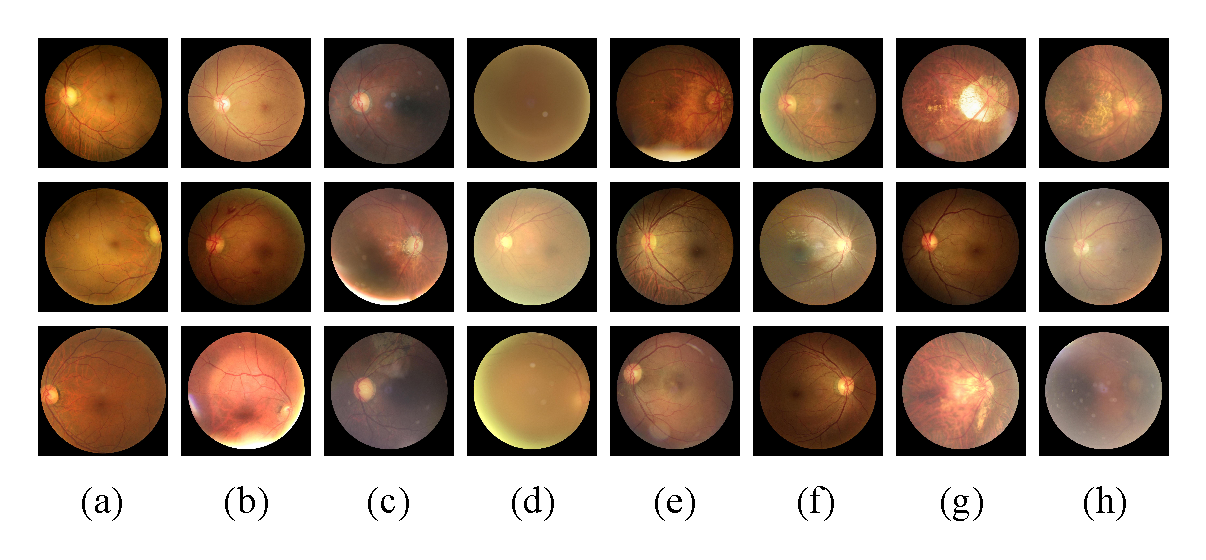
\includegraphics[width=0.86\textwidth]{./images/media/image5_padded.pdf}
\caption{ODIR 数据集中 8 类典型眼底图像示例}
\label{fig:odir-samples}
\end{figure}

为全面评估模型的域泛化能力，除ODIR域内泛化测试外，本文额外引入RIADD挑战赛提供的RFMiD\hyperref[_Ref213949409]{{[}47{]}}数据集作为第一个独立外部测试集。RFMiD包含3200张彩色眼底图像，原始训练集、验证集和测试集分别包含1920、640和640张图像，涵盖45种视网膜疾病或异常，由专业视网膜专家标注。其45类标签中含有部分与ODIR的8类标签重合的类别，这为模型泛化提供了基础。\figsubref{fig:rfmid-samples}{a}到\figsubref{fig:rfmid-samples}{h}选择性地展示了45种类别中的8类图像。考虑到RFMiD与ODIR的完整标签空间并不一致，本文选取二者共有的糖尿病视网膜病变（D）、年龄相关性黄斑变性（A）和病理性近视（M）三类进行跨数据集评估。在该设置下，ODIR侧构建得到1907张D/A/M三类训练图像，其中D、A、M的样本数分别为1425、255和253；RFMiD侧使用验证集中的119张三类图像进行外部测试，其中D、A、M的标签数分别为83、24和21。

\begin{figure}[!htb]
\centering
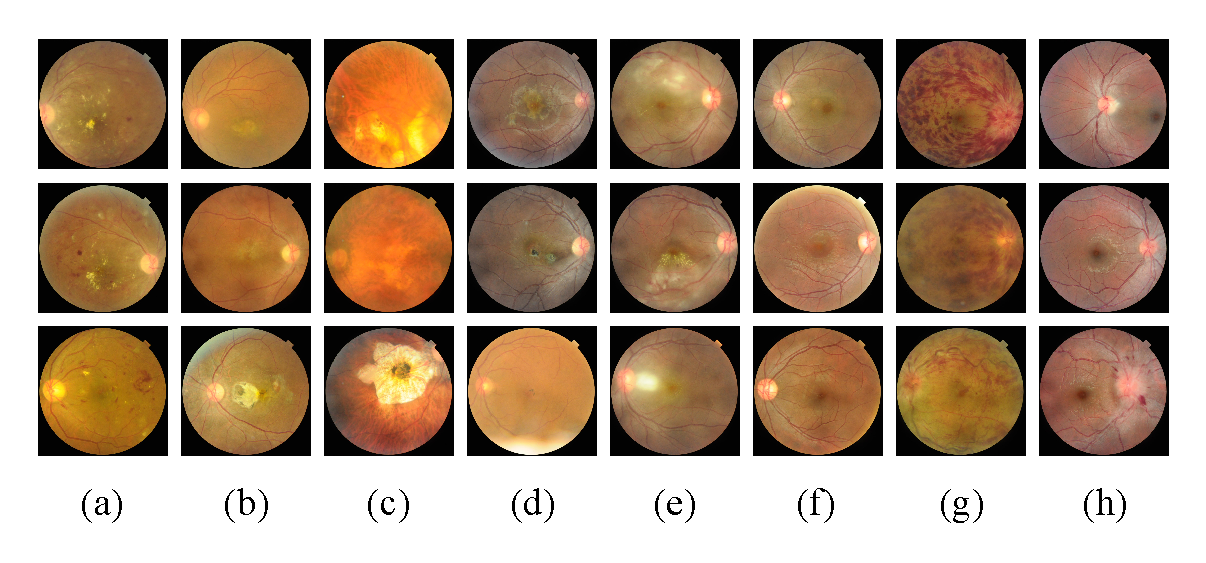
\includegraphics[width=0.86\textwidth]{./images/media/image6_padded.pdf}
\caption{RFMiD 数据集中选取的 8 类典型眼底图像示例}
\label{fig:rfmid-samples}
\end{figure}

此外，本文引入来自于 Anawara Hamida 和 B.N.S.B. Zahurul Haque 眼科医院采集的EDID\hyperref[_RefEDID2024]{{[}48{]}}数据集作为第二个独立外部测试集，以进一步验证所提方法在不同数据来源和不同标签组织方式下的泛化性能。EDID原始数据共包含5335张眼底图像，覆盖10个单标签类别，包括中心性浆液性脉络膜视网膜病变、糖尿病视网膜病变、视盘水肿、青光眼、健康眼底、黄斑瘢痕、近视、翼状胬肉、视网膜脱离和视网膜色素变性，对应样本数分别为101、1509、127、1349、1024、444、500、17、125和139。\figsubref{fig:edid-samples}{a}到\figsubref{fig:edid-samples}{h}展示了EDID数据集中选取的8类典型眼底图像示例。

\begin{figure}[!htb]
\centering
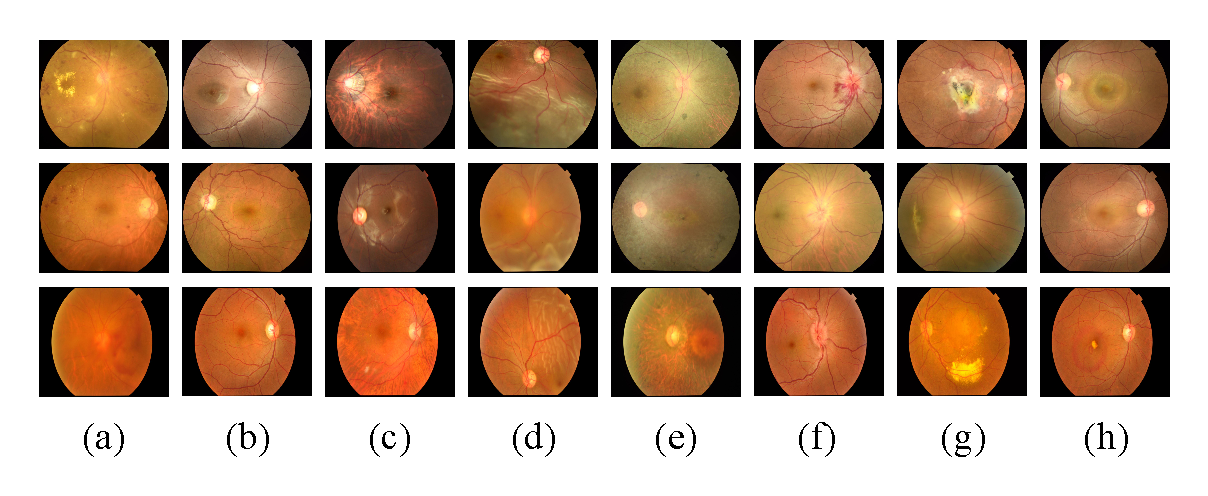
\includegraphics[width=0.86\textwidth]{./images/media/edid_samples_padded.pdf}
\caption{EDID 数据集中选取的 8 类典型眼底图像示例}
\label{fig:edid-samples}
\end{figure}

与RFMiD类似，考虑到EDID与ODIR的完整标签空间并不一致，本文选取二者共有的糖尿病视网膜病变（D）、青光眼（G）和病理性近视（M）三类构建外部测试集，共得到3358张图像，其中D、G、M的样本数分别为1509、1349和500。由于EDID为单标签数据集，本文将其视为多标签任务中的一种特殊情形，即每张图像仅有一个阳性标签，并在D/G/M三类空间下进行外部泛化评估。相应地，在ODIR侧构建D/G/M三类训练子集，共包含1871张图像，其中D、G、M的样本数分别为1401、227和243。

\letteredsubsection{B. 实验设置}
所有实验均以ResNet-50作为骨干网络，并在PyTorch框架下实现。评估指标沿用ODIR官方标准：Kappa系数、F1、AUC以及三者平均值Final score。Kappa阈值固定为0.5，F1采用micro平均方式以缓和类别不平衡影响。

对于基准框架，我们参考ODIR原始的ResNet-50的实现，并在此基础上进行了改进：原论文采用双目样本成对输入，尝试不同的特征层融合策略（如concat、prod、sum）后接8个独立的分类头进行患者级预测。我们的基准框架改为单眼图像为输入样本，样本同时带有所属患者的编号，分类器统一为单个多标签分类头，输出8维logits后经Sigmoid激活得到各疾病概率，损失函数为标准二元交叉熵（BCE）。推理阶段，将同一患者左右眼的单眼预测结果按逻辑合并得到患者级预测，从而与官方指标完全对齐。该改进避免了特征融合带来的噪声放大和个体差异信息稀释，尤其在双眼病变程度不一致时更有优势。

训练配置如下：优化器选择Adam，初始学习率\(1 \times 10^{-5}\)，采用OneCycleLR调度策略（前10\%轮次线性升温至峰值\(1 \times 10^{-5}\)，有助于模型快速跳出局部最优，后90\%轮次退火，有助于收敛和找到更优解），训练epoch为50，batch size为32，输入分辨率为448×448。所提框架在2张RTX 4080 Super上完成训练。后续实验结果表明，我们的改进基准框架（Off-set双目Final score 76.19）比起ODIR原文实现（Off-set双目Final score 68.00）能达到更好的效果。

\letteredsubsection{C. 与现有方法对比}

为评估所提方法在ODIR数据集上的分类性能，我们选取了四个典型的多标签眼科疾病分类方法，包括ODIR数据集论文提供的官方基线（Li et al.\hyperref[_Ref213949402]{{[}46{]}}）以及三项后续工作（Gour and Khanna、He et al.、Ou et al.）。这些方法主要聚焦于提升Final score，未考虑跨域泛化或隐私保护。

Gour and Khanna\hyperref[_Ref214903299]{{[}49{]}}提出基于转移学习的CNN框架，骨干网络采用VGG16，通过数据增强方法扩充ODIR数据集，然后采用SGD优化器细调模型，焦点在于利用预训练权重捕捉血管、视盘、黄斑等结构异常，以提升多类共存场景的识别性能。

He et al.\hyperref[_Ref213950338]{{[}20{]}}开发密集相关网络（DCNet），包括骨干CNN提取双眼特征、空间相关模块捕捉像素级相关性，以及分类器生成患者级分数。核心原理是通过密集卷积块融合左右眼特征，建模DR与AMD等疾病共现，但需依赖双目输入。

Ou et al.\hyperref[_Ref214903327]{{[}50{]}}设计双流交互CNN，使用特征增强模块通过注意力机制捕捉双眼局部-全局依赖，并多尺度模块叠加不同分辨率特征以丰富表示。其原理在于利用双流交互强化病变区域（如微血管瘤、出血点），提升多标签预测，但未考虑隐私或跨域场景。

\tabref{tab:sota-compare}报告了Off-set和On-set测试集上的双目指标对比，对比结果显示，所提方法在Off-set集的Final score为78.85，领先BFENet 0.85；在On-set集为77.49，领先BFENet 0.79。该结果证明了双分支引导特征学习与自适应标签关联构建在ODIR多标签识别任务中的有效性。

% Chapter 4 Experiments - Table 2
% Comparison with existing methods on Off-set and On-set.
\begin{table}[!htb]
\centering
\caption{与现有方法在 Off-set 和 On-set 上的对比}
\label{tab:sota-compare}
\resizebox{\textwidth}{!}{
\begin{tabular}{lcccccccc}
\toprule
\multirow{2}{*}{Method} & \multicolumn{4}{c}{Off-set} & \multicolumn{4}{c}{On-set} \\
\cmidrule(lr){2-5}\cmidrule(lr){6-9}
& Kappa & F1 & AUC & Final & Kappa & F1 & AUC & Final \\
\midrule
Li et al. & 35.45 & 84.83 & 83.72 & 68.00 & 36.97 & 85.35 & 84.08 & 68.80 \\
Gour and Khanna & 43.30 & 85.30 & 84.90 & 71.20 & 42.00 & 84.90 & 83.40 & 70.10 \\
He et al. & 52.00 & 88.60 & 90.30 & 77.00 & 50.00 & 87.70 & 89.70 & 75.80 \\
Ou et al. & 53.50 & 89.20 & 91.20 & 78.00 & 51.30 & 88.60 & 90.30 & 76.70 \\
\textbf{Ours} & \textbf{57.05} & \textbf{89.03} & \textbf{90.48} & \textbf{78.85} & \textbf{54.03} & \textbf{88.38} & \textbf{90.07} & \textbf{77.49} \\
\bottomrule
\end{tabular}
}
\end{table}


需要指出的是，现有对比方法主要围绕ODIR内部多标签分类指标进行优化，较少同时考虑域泛化和隐私保护。相比之下，本文除在ODIR Off-set和On-set上取得更高Final score外，还在RFMiD和EDID两个外部数据集上验证了未知域性能，并进一步评估隐私保护训练下的性能衰减。上述结果共同说明，所提框架不仅追求单一数据集上的分类精度，也面向更贴近临床部署的数据共享受限和隐私约束场景。

\letteredsubsection{D. 消融实验结果}
为系统验证所提框架中两大核心模块，即双分支引导域不变特征提取（DFE）与自适应标签-特征关联性构建（ARC）的独立贡献及协同增益，同时考察CAM引导对模型可解释性的提升，我们在ODIR Off-set双目指标上进行了逐模块消融实验，结果如\tabref{tab:ablation}所示。

% Chapter 4 Experiments - Table 3
% Ablation study of DFE and ARC modules.
\begin{table}[!htb]
\centering
\caption{消融实验结果。表中报告了在 ODIR Off-set 测试集下的双目指标。结果显示，DFE 和 ARC 相比 ResNet50（baseline）在 Final score 上均带来性能提升，分别提升 2.18 和 0.79；二者协同后进一步取得更高的指标提升，总体提升 2.66，并在四项指标上达到最佳结果，体现了两模块之间的正向协同作用。}
\label{tab:ablation}
\begin{tabular}{lcccc}
\toprule
Model & Kappa & F1 & AUC & Final \\
\midrule
ResNet50 & 52.75 & 87.83 & 88.00 & 76.19 \\
ResNet50+DFE & 56.20 & 88.80 & 90.10 & 78.37 \\
ResNet50+ARC & 53.19 & 87.45 & 90.29 & 76.98 \\
\textbf{ResNet50+DFE+ARC (Ours)} & \textbf{57.05} & \textbf{89.03} & \textbf{90.48} & \textbf{78.85} \\
\bottomrule
\end{tabular}
\end{table}


\begin{itemize}
\item
  纯ResNet-50基线：仅使用单分支ResNet-50与标准多标签分类头，Final score为76.19，Kappa为52.75，AUC是88.00。
\item
  ResNet50+DFE：仅引入完整的双分支引导域不变特征提取模块，Final score提升至78.37（+2.18），Kappa提升3.45，AUC提升2.10。性能提升主要源于CAM引导残差加权与掩码机制有效抑制了域特定噪声，使模型更关注可迁移的疾病相关特征，是整体性能提升的重要来源。如\figref{fig:cam-visualization}可视化结果显示，CAM热力图对图像边缘、光照伪影的关注减少，关注区域更收敛到眼球、血管等核心疾病区，模型可解释性增强。

\begin{figure}[!htb]
\centering
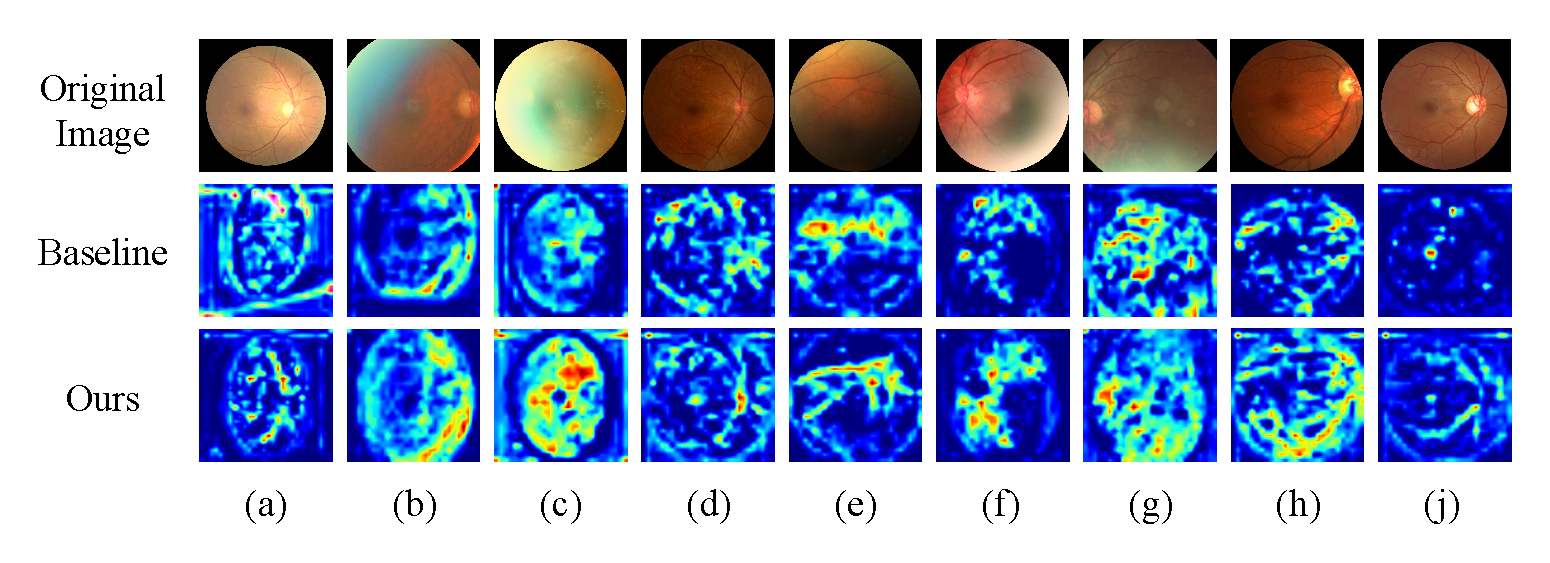
\includegraphics[width=0.92\textwidth]{./images/media/image8_padded.pdf}
\caption{基线方法与所提方法的 CAM 可视化对比}
\label{fig:cam-visualization}
\end{figure}

\item
  ResNet50+ARC：仅引入自适应标签-特征关联性构建模块，Final score提升至76.98（+0.78），Kappa提升0.44，AUC提升2.29。该模块通过显式建模疾病共现关系（如DR与AMD、近视与视盘异常）降低了漏检率，多标签分类性能提高。
\item
  ResNet50+DFE+ARC（完整框架，ours）：同时启用两大模块协同后，Final score进一步升至78.85（较基线+2.66），Kappa达到57.05（+4.30），F1与AUC分别达到89.03（+1.20）和90.48（+2.48）。总增益与两模块增益之和接近（2.66 \textless{} 2.18+0.78=2.96），体现了两模块之间的正向协同：DFE为ARC提供更稳定的疾病相关特征，使Transformer能更精准地学习标签依赖与特征-标签匹配；ARC的一致性损失反过来进一步约束双分支输出分布，提升特征表示的稳定性。
\end{itemize}

消融结果证明：自适应标签-特征关联性构建（ARC）验证了标签关联建模对多疾病共存场景的有效性，双分支引导域不变特征提取（DFE）验证了在多机构联合训练难以满足时，仅利用单一源域学习可迁移疾病相关特征的必要性。两模块的深度融合协同使得所提框架在仅使用单域数据训练的情况下进一步提升多标签识别性能，并为后续跨域泛化结果提供支撑，体现了本方法设计的科学性与高效性。

\letteredsubsection{E. 泛化性能结果}

为全面验证所提框架在单域训练条件下的泛化能力以及隐私保护机制的有效性，我们分别在非隐私和隐私保护两种场景下进行了系统性评估，涵盖ODIR内部测试（Off-set与On-set）和外部跨数据集测试（RFMiD与EDID）。



（1）非隐私条件下的泛化性能 结果如\tabref{tab:generalization}所示，表中报告了基线与所提方法在不同测试集上的Final score。泛化实验按三个评估方向组织：ODIR内部的Off-set \(\rightarrow\) On-set、ODIR到RFMiD的外部泛化，以及ODIR到EDID的外部泛化。每个方向均基于训练过程中保存的前5个候选权重进行模型选择与评估，即分别在Base和Ours的候选权重中确定目标测试集表现最优的一组权重，并同步报告该组权重在源域Off-set和目标测试集上的结果。

% Chapter 4 Experiments - Table 4
% Generalization performance on ODIR, RFMiD/RIADD, and EDID.
\begin{table}[!htb]
\centering
\caption{不同测试集上的泛化性能比较。比较了 Baseline 与 Ours 在 ODIR 内部泛化（Off-set $\rightarrow$ On-set）以及 ODIR 到 RFMiD、EDID 外部泛化中的表现，比较的指标均为Final score。其中，Off-set $\rightarrow$ On-set 同时报告了单目与双目结果，外部泛化部分报告了各数据集对齐三类标签空间后的单目结果；每个方向均在候选权重中选择目标测试集表现最优的模型进行报告。总体上，所提方法在各测试方向上均优于基线。}
\label{tab:generalization}
\resizebox{\textwidth}{!}{
\begin{tabular}{lcccccccc}
\toprule
\multirow{3}{*}{Model} & \multicolumn{4}{c}{Off-set $\rightarrow$ On-set} & \multicolumn{2}{c}{Off-set $\rightarrow$ RFMiD} & \multicolumn{2}{c}{Off-set $\rightarrow$ EDID} \\
\cmidrule(lr){2-5}\cmidrule(lr){6-7}\cmidrule(lr){8-9}
& \multicolumn{2}{c}{Off-set} & \multicolumn{2}{c}{On-set} & Off-set & RFMiD & Off-set & EDID \\
\cmidrule(lr){2-3}\cmidrule(lr){4-5}\cmidrule(lr){6-7}\cmidrule(lr){8-9}
& Monocular & Binocular & Monocular & Binocular & Monocular & Monocular & Monocular & Monocular \\
\midrule
ResNet50 & 79.37 & 76.19 & 77.30 & 75.23 & 94.39 & 83.86 & 94.30 & 52.16 \\
\textbf{Ours} & \textbf{81.71} & \textbf{78.79} & \textbf{78.98} & \textbf{77.49} & \textbf{95.94} & \textbf{85.06} & \textbf{96.03} & \textbf{55.35} \\
\bottomrule
\end{tabular}
}
\end{table}


在ODIR内部泛化测试中，目标测试集为On-set，\tabref{tab:generalization}同时报告单目（Monocular）和双目（Binocular）两种评估方式。ResNet-50基线对应权重在Off-set和On-set上的双目指标分别为76.19和75.23，而所提方法对应权重将指标提升至78.79和77.49，增幅分别达2.60和2.26个百分点；单目指标同样由79.37和77.30提升至81.71和78.98。这说明双分支引导特征学习与CAM引导注意力能够增强模型对疾病相关区域的关注。其中双目指标低于单目指标的原因是，模型本身以单目数据进行训练，推理阶段将同一患者左右眼预测结果合并时，任一只眼的错误预测都可能影响患者级判断，从而放大单眼小错误对最终指标的影响。

在外部跨数据集测试中，RFMiD和EDID与ODIR的完整标签空间并不一致，因此本文先重构共有三类标签空间，再进行泛化评估。其中RFMiD实验对齐D/A/M三类，EDID实验对齐D/G/M三类；EDID虽然为单标签数据集，但同样可在三类共有标签空间下作为外部泛化测试集。考虑到外部数据集与ODIR在成像设备、采集流程、光照条件、疾病组成和标签定义上存在更明显差异，本文同样基于前5个候选权重进行模型选择与评估，并同步报告该组权重在三类ODIR Off-set和目标数据集上的单眼Final score。

结果显示，在RFMiD D/A/M外部泛化实验中，Base对应权重的ODIR Off-set分数为94.39，目标域Final score为83.86；所提方法对应权重的ODIR Off-set分数为95.94，目标域Final score为85.06，分别提升1.55和1.20个百分点。进一步从细分指标看，所提方法在RFMiD上的Kappa、F1和AUC分别为73.95、87.96和93.27，均高于Base的72.08、87.11和92.39。在EDID D/G/M外部泛化实验中，Base对应权重的ODIR Off-set分数为94.30，目标域Final score为52.16；所提方法对应权重的ODIR Off-set分数为96.03，目标域Final score为55.35，分别提升1.73和3.19个百分点。所提方法在EDID上的Kappa、F1和AUC分别为27.20、67.22和71.63，较Base的23.83、65.54和67.09均有提升。综合来看，RFMiD结果验证了模型在多标签外部数据集上的跨域泛化能力；EDID结果进一步说明，在单标签外部数据集被纳入三类泛化评估框架的情况下，所提方法仍能保持有效提升。

（2）自适应高斯差分隐私超参数扫描 结果如\tabref{tab:privacy-scan}所示。引入隐私保护后，噪声注入速率会一定程度影响模型收敛行为与最终性能。实验发现，初始噪声乘数（noise\_multiplier）与衰减速率（noise\_decay\_rate）共同决定了噪声注入曲线：过强的初始噪声会导致训练剧烈震荡甚至不收敛，而过快的衰减则使隐私预算在模型尚未充分学习时提前耗尽。其中，setting1（noise\_multiplier=0.65）提供了极强的隐私保护，但因初始噪声过大，导致\(\epsilon\)值仅为5.01，使模型性能严重下降；setting8（noise\_multiplier=0.25，decay\_rate=4e-6）虽然使得模型性能接近非隐私情况，但是\(\epsilon \approx 20\)隐私保护弱。综合性能与隐私预算，我们最终选取setting5（noise\_multiplier=0.35，decay\_rate=4e-6），在80 epoch后\(\epsilon \approx 10.15\)，实现了隐私强度与模型可用性的最佳折衷。

% Chapter 4 Experiments - Table 3
% Hyperparameter scan for adaptive Gaussian differential privacy.
\begin{table}[htbp]
\centering
\caption{自适应高斯差分隐私超参数扫描结果}
\label{tab:privacy-scan}
\begin{tabular}{lccc}
\toprule
Setting & noise\_multiplier & noise\_decay\_rate & $\epsilon$ / 80 epoch \\
\midrule
setting1 & 0.65 & 1.5e-6 & 5.01 \\
setting2 & 0.50 & 2e-6 & 6.80 \\
setting3 & 0.40 & 4e-6 & 8.71 \\
setting4 & 0.35 & 2e-6 & 9.96 \\
setting5 & 0.35 & 4e-6 & 10.15 \\
setting6 & 0.30 & 2e-6 & 11.91 \\
setting7 & 0.25 & 2e-6 & 15.11 \\
setting8 & 0.25 & 4e-6 & 20.01 \\
\bottomrule
\end{tabular}
\end{table}


（3）隐私训练过程中的\(\epsilon\)-性能演化与优化策略 结果如\tabref{tab:privacy-evolution}所示。采用setting5的噪声速率后，我们记录了训练过程中\(\epsilon\)消耗与单目指标的逐epoch变化。结果显示，随着\(\epsilon\)从第0轮的0.94逐步增长至第79轮的10.15，隐私逐步消耗，模型性能持续提升，至第74轮附近达到峰值（Final=73.15）。这表明自适应衰减策略允许模型在隐私预算内充分学习。取第74轮的模型权重是兼具隐私保护和性能的平衡点。经过大量实验验证，隐私场景需对优化策略进行针对性调整：

% Chapter 4 Experiments - Table 6
% Epsilon-performance evolution during privacy training.
\begin{table}[!htb]
\centering
\caption{隐私训练过程中 $\epsilon$ 与性能的演化。表中使用的是\tabref{tab:privacy-scan}中 setting5 的加噪策略，评估指标是单目下的Final score，随着训练推进，隐私预算逐步消耗、模型性能总体上升，并在 e74 达到峰值（红色部分）。此权重将作为本文在隐私约束下采用的最佳性能检查点。}
\label{tab:privacy-evolution}
\begin{tabular}{lccccc}
\toprule
Epoch & $\epsilon$ & Kappa & F1 & AUC & Final \\
\midrule
e0 & 0.94 & 29.39 & 84.70 & 78.70 & 64.26 \\
e10 & 3.28 & 34.24 & 85.77 & 81.27 & 67.09 \\
e22 & 4.91 & 36.42 & 85.85 & 82.83 & 68.36 \\
e31 & 5.91 & 39.70 & 86.28 & 83.56 & 69.85 \\
e40 & 6.81 & 40.62 & 86.13 & 84.08 & 70.28 \\
e49 & 7.65 & 40.64 & 87.01 & 85.17 & 70.94 \\
e52 & 7.92 & 42.16 & 87.46 & 85.00 & 71.54 \\
e64 & 8.94 & 42.45 & 87.38 & 85.89 & 71.91 \\
e68 & 9.27 & 43.59 & 87.76 & 86.18 & 72.51 \\
\textcolor{red}{e74} & \textcolor{red}{9.76} & \textcolor{red}{45.12} & \textcolor{red}{87.91} & \textcolor{red}{86.42} & \textcolor{red}{73.15} \\
e79 & 10.15 & 43.16 & 87.51 & 86.47 & 72.38 \\
\bottomrule
\end{tabular}
\end{table}


1. 学习率从\(1 \times 10^{-5}\)提升至\(7.5 \times 10^{-5}\)。

2. 学习率调度改为``先线性衰减后恒定''： 以lr\_decay\_ratio和lr\_final\_factor控制衰减轮次和衰减比例，所取值分别为0.75和0.8，即学习率在前75\%轮次内线性衰减至原值的80\%，之后保持恒定训练。

原因在于，隐私情况下的模型训练和常规情况下的模型训练不一样。对于学习率的取值来说，隐私情况下，每一次回传的梯度中都会叠加噪声，这使得每一次模型优化时的损失值在原基础上波动，增大了陷入局部最优的概率，因此学习率需要适当增大。对于学习率调度策略，在常规情况下当模型收敛到最优值附近时，非隐私训练的学习速率通常会逐步减小；相比之下，隐私情况下的学习过程不需要将学习率降低到一个非常小的值，因为差分隐私训练会以隐私消耗不断增大的代价持续优化，却未必真正达到模型收敛。因此，以相对较大的学习率开始，然后在一定周期内线性衰减到较小的值，并在之后保持恒定，性能会更好。

实验证明，该策略改善了收敛稳定性，最终在\(\epsilon = 9.76\)时取得了73.15的Final score，明显优于固定噪声或低学习率配置。

（4）隐私保护下的最终泛化性能 结果如\tabref{tab:privacy-final}所示。最优隐私模型在ODIR同域双目指标上的Off-set和On-set Final score分别为68.96和68.42，相较无隐私版本下降约10个百分点，但已接近或略优于ODIR原文官方基线（68.8），实现了在中等隐私预算下与公开基准持平的性能，充分体现了自适应高斯差分隐私机制的有效性。

% Chapter 4 Experiments - Table 7
% Final generalization performance under privacy mode.
\begin{table}[!htb]
\centering
\caption{隐私保护下的泛化性能对比。表中报告 ODIR 同域双目 Final score，其中 Ours（privacy）采用的是\tabref{tab:privacy-evolution}中选取的最优隐私权重。在中等隐私预算下，所提方法在 Off-set 上略优于 Li et al. \hyperref[_Ref213949402]{{[}46{]}} 报告的官方基线，并在 On-set 上保持接近性能。}
\label{tab:privacy-final}
\begin{tabular}{lcc}
\toprule
Model & Off-set & On-set \\
\midrule
Li et al. \hyperref[_Ref213949402]{{[}46{]}} & 68.00 & 68.80 \\
\textbf{Ours (privacy)} & \textbf{68.96} & \textbf{68.42} \\
\bottomrule
\end{tabular}
\end{table}

